%A pointform description of the general idea
%\begin{itemize}
%	\item A D-NURBS approach to simulation. Use a Jacobian to map from UV positions in a NURBS parametric space to world space positions on the surface. 
%	\item \textbf{Shape Matching}: From the sample world space positions on a single NURBS surface, we solve a least squares problem to fit a \textit{projection operator} to the surface. This projection operator maps monomials in the undeformed space, to the least squares estimate of the deformed positions for the given monomials.
%	\item With DNURBS and Shape Matching VEM we have two mappings: a UV to undeformed world space with our NURBS Jacobian, then an undeformed to deformed mapping with the projection operators. This lets us form a set of generalized coordinates in terms of our control points of the NURBS surface (section 1.4).
%	\item For an arbitrary position in space (not necessarily on the surface), we can build a projection operator unique to this point via a weighted sum of the projection operators of the projection operators for each NURBS (eq 5). From this we can reconstruct an estimate of the deformed position from the monomial basis defined using its undeformed position.
%	\item For any point in space, we need to compute a set of weights to the projection operators defined on the surfaces with the following criteria: the weights sum to 1, are nonzero, and depend on the distances to the surfaces (See section 1.8).
%	\item With this mapping for undeformed to deformed positions, this yields a simple definition for the deformation gradient (eq 12).
%	\item Armed with our deformation gradient, we next define the Lagrangian, but this basic form isn't sufficient. We augment our kinetic and potential energies with a stability term (ref VEM). This accounts for cases in which the position of the nodal values don't match their estimated positions defined by the projection operator mapping.
%	\item \textbf{Raycasting Quadrature}: To compute the volume integrals we make use of raycasting quadrature approach (ref) where we uniform sample a YZ grid and shoot rays in the X direction. We then use the points of intersection to define integrations bounds for 1D integrals along these rays, which we integrate numerically.
%	\item With our augmented lagrangian, we use the Euler-Lagrange equation to arrive at equations of motion. Our generalized coordinates give us direct updates on the control points of the NURBS. Currently we are using linearly-implicit Euler for time integration.
%	\item \textbf{Handling trimmed NURBS}: For this case we update the original control points, but we must only sample points within the boundary. To compute these points we use an approach similar to the raycasting quadrature but in 2D. In the paremtric domain for a T-NURBS we sample uniforly in the V direction and shoot rays along the U axis. At each region of intersection, we sample more values along the ray. The final result is a set of UV coordinates that respect the boundary defined by NURBS curves.
%\end{itemize}


\section{Methods}
Brief overview. We have some control points. We have UV samples on the NURBS parametric domain. We have a NURBS jacobian UV to points on surface in R3.
Given a volumetric model composed of one or more NURBS surfaces, the surface of each surface is reconstructed using a set of control points $\textbf{p}$ and their associated weights $w$. Following D-NURBS \cite{10.1145/176579.176580}, we take our degrees of freedom (DOF) to be control points of the surfaces and produce displacements directly on these control points at each simulation step. We note that we used a simplified version of D-NURBS in which the weights are held constant throughout the simulation and find this not to be limiting \myworries{(feel like we'll need better justification than saying just this?)}. We represent the degrees of freedom for the $i$-th NURBS surface with $m$ control points as $\mathbf{q}_i = \left[ \mathbf{p}_1^T, \dots, \mathbf{p}_m^T \right]^T \in \mathbb{R}^{3m}$. From this definition, we write the DOF for the entire model as $\mathbf{q} = \left[ \mathbf{q}_i^T, \dots, \mathbf{q}_n^T \right]^T$ where $n$ is the number of NURBS surfaces for the model. 

To evaluate the volumetric integrals in solid mechanics models, we require material points $\mathbf{X} \in \mathbb{R}^{3m}$ in the undeformed space that serve as integration points. Our shape matching element method enables us to evaluate the deformed positions of the material points strictly using positions defined on the boundary. Like in VEM, we fit a polynomial to each boundary primitive (NURBS in this case) describing its deformation. The fitting of these polynomials closely follows that of the Shape Matching \cite{10.1145/1073204.1073216} approach where we perform a least squares polynomial fit to the deformed boundary points. These boundary points are represented by sampled positions on each NURBS surface. Since each surface is associated with a single polynomial, we can construct a unique polynomial for some arbitrary point by blending these polynomials. Thus given some material point $\mathbf{X}_i$ we find it's corresponding deformed position $\mathbf{x}_i$ via a weighted combination of the polynomials. This permits us to build a general deformation map which we use to construct our equations of motion.

In the following sections, we will first review the simplified D-NURBS model used to form our generalized coordinates. We then present our shape matching algorithm for fitting polynomials to surfaces .... In section ... we next describe how to blend these surface polynomials to construct a general deformation map for material points. Section ... describes our strategy for selecting integration points in the volume through a raycasting approach. Finally, we formulate our equations of motions from a Lagrangian formulation.

\section{D-NURBS Model}
We provide a brief overview of the D-NURBS formulation presented in \cite{10.1145/176579.176580}. Our models in our method are composed of a collection of NURBS surfaces. 

\subsection{D-NURBS Formulation}
A point on a NURBS surface is typically expressed in the following form
\begin{equation}
\label{eqn:nurbs_srf}
    \mathbf{x}(u,v) = \frac{\sum_{i=1}^{n}\sum_{j=1}^{m}  \mathbf{p}_{i,j} w_{i,j} B_{i,k}(u)B_{j,l}(v)}
    {\sum_{i=1}^{n}\sum_{j=1}^{m} w_{i,j} B_{i,k}(u)B_{j,l}(v)}
    \text{,}
\end{equation}
where where have a total of $nm$ control points $\mathbf{p}$ and weights $w$. Using the B-spline basis functions and the weighted control points, this formula gives a map from our parametric coordinates $u,v$ to their corresponding position on the surface in $\mathbb{R}^{3m}$. $B_{i,k}(u)$ is the B-spline basis function for the $i-th$ control point with degree $k-1$.

We would like our generalized coordinates to be the control points of the model so that the dynamics operates directly on the original representation. Therefore, we would like to rewrite equation \ref{eqn:nurbs_srf} in the form
\begin{equation}
    \mathbf{x}(u,v) = \mathbf{J}(u,v)\mathbf{q}
    \text{,}
\end{equation}
where $\mathbf{q} = \left[ \mathbf{p}_{1,1}^T, \dots, \mathbf{p}_{i,j}^T, \dots, \mathbf{p}_{n,m}^T \right]^T \in \mathbb{R}^{3nm}$ is the set of $nm$ control points \myworries{in the overview I just write $n$ control points, but here i'm writing $nm$} for a single NURBS surface arranged as a column vector. $\mathbf{J} \in  \mathbb{R}^{3 x 3nm}$ is the NURBS jacobian that maps $(u,v)$ coordinates to world positions in $\mathbb{R}^{3}$.

The NURBS jacobian, $\mathbf{J}$, is a matrix composed of horizontally concatenated $3x3$ blocks where the $(i,j)$-th block is $\frac{\partial \mathbf{x}}{\partial \mathbf{p}_{i,j}}$ for the $(i,j)$-th control point. $\frac{\partial \mathbf{x}}{\partial \mathbf{p}_{i,j}}$ is a diagonal $3x3$ matrix where each diagonal entry $N_{i,j}(\mathbf{u})$ takes the form

\begin{equation}
\label{eqn:jacobian_diagonal}
    N_{i,j}(u,v)
    = \frac{w_{i,j} B_{i,k}(u)B_{j,l}(v)}{\sum_{i=1}^{n}\sum_{j=1}^{m} w_{i,j} B_{i,k}(u)B_{j,l}(v)}
    \text{.}
\end{equation}
Thus the NURBS jacobian for a single $(u,v)$ pair is written as
\begin{equation}
\label{eqn:uv_jacobian}
    \mathbf{J}(u,v)
    \left[ \frac{\partial \mathbf{x}}{\partial \mathbf{p}_{1,1}} \dots
           \frac{\partial \mathbf{x}}{\partial \mathbf{p}_{i,j}} \dots 
           \frac{\partial \mathbf{x}}{\partial \mathbf{p}_{n,m}}
    \right]
    \text{.}
\end{equation}

This formulation is a simplification of the full D-NURBS described in \cite{10.1145/176579.176580} the weights of the NURBS are fixed throughout the simulation. Permitting the dynamics to modify weights would likely improve the expressiveness of the kinematics, but we find fixing the weights affords sufficiently expressive results and improves performance. The performance improvement is a result of having fixed $N_{i,j}(u,v)$ entries over the course of the simulation. The full D-NURBS model requires rebuilding the jacobian and consequently the mass matrices at each time step. 

\subsection{Generalized Coordinates for a NURBS model}
The above formulation describes developing the map from a single $(u,v)$ coordinate to its corresponding position on the surface. In our simulation we represent the entire boundary of the NURBS model, so we require samples along each surface. We emphasize that we only require an initial selection of $(u,v)$ coordinates across each surface and the dynamics of the simulation modifies the set of control points $\mathbf{q}$ to modify the world space maps $\mathbf{x}(u,v)=\mathbf{J}(u,v)\mathbf{q}$.

Let's say for a NURBS surface on the model the DOF column vector is $\mathbf{q}_i$, which is the subset of control points in the generalized coordinates for the $i$-th surface. For a given surface with $m$ pairs of $\mathbf{u}=(u,v)$ coordinates sampled in parametric space, we write the jacobian for the $i$-th surface as \myworries{(should I use something like $\hat{\mathbf{J}}$ instead?)}
\begin{equation}
\label{eqn:surface_jacobian}
    \mathbf{J}_i =
    \left[ \mathbf{J}(\mathbf{u})_1^T \dots \mathbf{J}(\mathbf{u})_m^T \right]^T
    \text{.}
\end{equation}
Then if $\mathbf{x}_i$ is the set of $m$ world space positions for the $i$-th surface, we may write $\mathbf{x}_i = \mathbf{J}_i \mathbf{q}_i$. Finally, given the full set of generalized coordinates $\mathbf{q} = \left[ \mathbf{q}_i^T, \dots, \mathbf{q}_n^T \right]^T$ with $n$ surfaces, we may write jacobian $\mathbf{J}$ for the entire model as a block diagonal matrix:
\begin{equation}
\mathbf{J} = \left( \begin{array}{ccccc}
\mathbf{J}_1 &  &  &  &  \\
 & \ddots &  &  &  \\
 &  & \mathbf{J}_i & &  \\
 &  &  & \ddots &  \\
 &  &  &  & \mathbf{J}_n \\
\end{array} \right)
\end{equation}
With this equation, the full set of world positions of the NURBS model may be written as $\mathbf{x} = \mathbf{J}\mathbf{q} \in \mathbb{R}^{3N}$ where $N$ is the total number of $(u,v)$ coordinates.

\section{Shape Matching}
\section{Blending Polynomials}
\section{Raycasting Quadrature}
\section{Dynamic Simulation}
\subsection{Generalized Inertia}
\subsection{Generalized Forces}
\subsection{Equations of Motion}
%This is most notable in cases where the degree of the polynomial on a NURBS is higher than the degree of the B-spline surface.

%

% \textbf{x}(\textbf{X}) = \hat{A}M(\textbf{X}) + \bar{\textbf{x}}$ \\
% $\hat{A} = \sum_i^{|S|}w_i(\textbf{X})A_i$
%
%
%In our case, the function we are trying to evaluate is deformation with respect to the center of mass. In VEM, instead of reconstructing values of our function using nodal values, we seek to find a a set of polynomial coefficients that map some arbitrary undeformed position to a polynomial approximation of its deformed position. This set of polynomial coefficients is referred to as the projection operator, $\mathbf{\Pi}$. The key point here is that $\mathbf{\Pi}$ is constructed strictly using positions defined on the boundary, avoiding the need for explicit representation of the interior. \\
%
%\subsection{Shape Matching: }
%In shape matching, authors seek a polynomial transformation, $\mathbf{\Pi}$ that minimizes $\sum_i ||\mathbf{\Pi}\mathbf{M(X)} - \mathbf{p_i}||^2$ where $\mathbf{M(X)}$ is the monomial basis of the $i$-th boundary vertex and $\mathbf{p_i}$ is current displacement from the center of mass for the $i$-th point. We argue this paper can be interpreted as a sort of virtual element method. \\
%
%\subsection{Reconstructing deformed positions}
%A general form for the monomial basis takes the following form <insert here>. For example, in 2D with quadratic deformation we have:
%\begin{equation}
%    \mathbf{M(X)} =\begin{bmatrix}
%    X_0 - \bar{X}_0  \\ 
%    X_1 - \bar{X}_1  \\ 
%    (X_0 - \bar{X}_0)^2  \\ 
%    (X_1 - \bar{X}_1)^2  \\ 
%    (X_0 - \bar{X}_0)(X_1 - \bar{X}_1) 
%    \end{bmatrix} 
%\end{equation}
%
%    
%We write the estimated deformed position $\mathbf{x}$ of some arbitrary undeformed position $\mathbf{X}$ as
%\begin{equation}
%     \mathbf{x}(\mathbf{X}) = \hat{\mathbf{\Pi}}\mathbf{M}(\mathbf{X}) + \bar{\mathbf{x}} 
%\end{equation}
%where $\mathbf{\hat{\Pi}}$ is the blended projection operator for this particular point:
%\begin{equation}
%    \hat{\mathbf{\Pi}}\mathbf{(X)} = \sum_i^{|S|}w_i(\mathbf{X})\mathbf{\Pi}_i 
%\end{equation}
%The bar symbol indicates the center of mass. For example, $\bar{\mathbf{x}}$ is the deformed object's center of mass, which we compute as the mean of the boundary values 
%\begin{equation}
%    \bar{\mathbf{x}} = \frac{1}{n}\sum_i^n x_i 
%\end{equation}
%Here $w_i$ is some weighting function for the $i$-th shape. There are many possible forms for this weighting function. Right now we compute these weights by forming the following optimization: \\
%<insert here>
%In order to form the equations of motion, we need to re-express the above equation in terms of the nodal values, $\mathbf{q}$. To arrive it these we note that each $\mathbf{\Pi}_i$ is a function of $\mathbf{q}$. 
%\begin{equation}
%    \mathbf{\Pi}_i(\mathbf{q}) = \mathbf{P(E_i q)M(E_i q_0)^{\dagger}}
%\end{equation}
%\myworries{I'm not a fan of what I wrote here. The MLS-MPM paper presents a similar idea when talking about EFG, and I like their notation a bit better}
%This is the shape matching problem's least squares solution where $M(q_0)^{\dagger}$ is the Moore-Penrose pseudo-inverse of the monomial vectors stacked row-wise (add example equation). The matrix $\mathbf{E}_i$ selects the degrees of freedom from $\mathbf{q}$ associated with the $i$-th shape. The function $\mathbf{P(q)}$ evaluates the displacement of these values from the current center of mass. We observe that the above equation is linear in $\mathbf{q}$ so we may rewrite the equation for $\mathbf{x}$ as 
%\begin{equation}
%    \mathbf{x(X)} = \mathbf{J_{\hat{\Pi}}(X)q}
%\end{equation}
%
%
%\subsection{Generalized Coordinates}
%With D-NURBs simulation layered on the VEM simulation, we have two Jacobians: $\mathbf{J}(u,v)$ mapping controls points, $\mathbf{p}$ onto surface positions, and then $\mathbf{J_{\hat{\Pi}}(X)}$ which maps surface positions $\mathbf{q}$ to their deformed positions. The Jacobian $\mathbf{J}(u,v)$  may be precomputed, and each point sampled on a surface of a NURBs has an associated $\mathbf{J}(u,v)$. With these two Jacobians we may express a single $u,v$ pair's deformed position as
%\begin{equation}
%    \mathbf{x}(u,v,\mathbf{p}) = \mathbf{J_{\hat{\Pi}}(X)}\mathbf{J}(u,v)\mathbf{p}
%\end{equation}
%and the undeformed position
%\begin{equation}
%    \mathbf{X}(u,v) = \mathbf{J}(u,v)\mathbf{p_0}
%\end{equation}
%where $\mathbf{p_0}$ is the initial values for the control points.
%
%\subsection{Deformation Gradient}
%\begin{equation}
%        \mathbf{F} = \frac{\partial \mathbf{x}}{\partial \mathbf{X}}
%               = \frac{\partial \hat{\mathbf{\Pi}}\mathbf{M(X)}}{\partial \mathbf{X}}
%               = \hat{\mathbf{\Pi}} \frac{\partial \mathbf{M(X)}}{\partial \mathbf{X}} 
%\end{equation}
%The $\frac{\partial \mathbf{M(X)}}{\partial \mathbf{X}}$ terms may be precomputed and using the previous $\mathbf{M(X)}$ example, we have
%\begin{equation}
%     \frac{\partial \mathbf{M(X)}}{\partial \mathbf{X}} = \begin{bmatrix}
%     1&0 \\ 
%     0&1 \\ 
%     2(X_0 - \bar{X}_0)&0 \\ 
%     0&2(X_1 - \bar{X}_1) \\ 
%     (X_1 - \bar{X}_1)&(X_0 - \bar{X}_0) 
%    \end{bmatrix}
%\end{equation}
%
%In computing the forces and the stiffness matrix, we require the gradient of the deformation gradient with respect to the configuration,  $\frac{\partial \mathbf{F}}{\partial \mathbf{q}}$. Usually the form of this gradient is simple. For example, in linear tetrahedral FEM each quadrature point's deformation map only involves the four surrounding nodal values, simplifying this gradient. In our case, the presence of the projection operator $\hat{\mathbf{\Pi}}$ means that each quadrature point is computed using the nodal values of the entire model. 
%
%\begin{equation}
%    \frac{\partial \mathbf{F}}{\partial \mathbf{q}} = \frac{\partial \mathbf{P}}{\partial q}\mathbf{M(q_0)}^\dagger  \frac{\partial \mathbf{M(X)}}{\partial \mathbf{X}} 
%\end{equation}
%
%
%Naively handled, this gives us a $\frac{\partial \mathbf{F}}{\partial \mathbf{q}}$ of size $3 x |q|$. However, many of the columns of have values all near zero, allowing us to prune many columns for each quadrature point. Currently, I'm computing the infinity norm of each column and prune all except some fixed number of columns. \\
%
%
%\subsection{Variational Mechanics}
%We have now provided all the necessary ingredient to produce equations of motion for deformable bodies, which we derive via Euler-Lagrange equation. We begin with the Lagrangian
%\begin{equation}
%    L=T-V
%\end{equation}
%where $T$ is the kinetic energy, and $V$ is the potential energy. From the Euler-Lagrange equation we have:
%\begin{equation}
%    \frac{d}{dt} \frac{\partial L}{\partial \dot{\mathbf{p}}} + \frac{\partial L}{\partial {\mathbf{p}}} = 0
%\end{equation}
%\begin{equation}
%    V =  \int_\Omega \psi(\mathbf{F(X)} dX
%\end{equation}
%then discretizing this over $m$ quadrature points, we have
%\begin{equation}
%    V =  \sum_i^m \psi(\mathbf{F(X_i)} A_i
%\end{equation}
%\begin{equation}
%    \frac{\partial L}{\partial \mathbf{q}} = \sum_i^m \frac{\partial V_i}{\partial \mathbf{q}} = \sum_i^m \frac{\partial \psi(\mathbf{F_i)}}{\partial \mathbf{F}}\frac{\partial \mathbf{F_i}}{\partial \mathbf{q}}A_i
%\end{equation}
%Next we have the equation of the kinetic energy
%\begin{equation}
%    T = \frac{1}{2}\int_{ \Omega} \rho \dot{\mathbf{x}}^T\dot{\mathbf{x}} dV
%\end{equation}
%which we rewrite in terms of our control points configuration
%\begin{equation}
%    T = \frac{1}{2} \int_{\partial \Omega} \dot{\mathbf{p}}^T \mathbf{J}(u,v)^T \mathbf{M} \mathbf{J}(u,v) \dot{\mathbf{p}} du dv
%\end{equation}
%\myworries{change notation to not use M for the monomial basis}
%where
%\begin{equation}
%    \mathbf{M} = \int_\Omega \rho \mathbf{J_{\hat{\Pi}}(X)}^T \mathbf{J_{\hat{\Pi}}(X)}
%\end{equation}
%From the potential energy (which uses dF/dq) and this potential energy, we discretize in time and right now I'm using linearly implicit backward euler
%
%\subsection{Stability term}
%\begin{figure}[h]
%  \centering
%  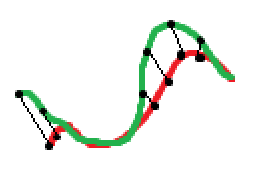
\includegraphics[width=\linewidth]{figures/error_energy}
%  \caption{A figure showing the spring energy error for each sampled point on the NURBS curve. I should change the colors of the lines to show higher energies where the error is higher.}
%  \Description{Showing an example error of a NURBS curve.}
%\end{figure}
%
%\subsection{Projection Operator Weighting}
%\begin{figure}[h]
%  \centering
%  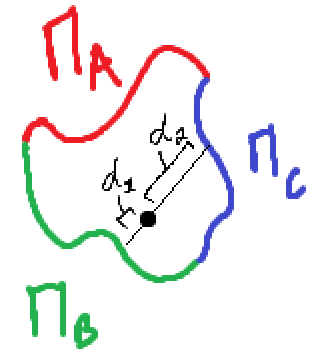
\includegraphics[width=\linewidth]{figures/distance_weighting}
%  \caption{A 2D example showing how $\theta$ is computed for $\Pi_B$. $d_1$ shows the distance to the closest point on $\Pi_B$ to $\mathbf{x}$ and $d_2$ shows the distance to the surface hit by the ray in the opposite direction.}
%  \Description{Showing a 2D NURBS curve with a quadrature point in the center. A ray is cast to the nearest point on a shape, showing the distance between the quadrature point and the nearest point as well as the distance to the "back surface".}
%\end{figure}
%
%\begin{equation}
%\begin{aligned}
%\mathbf{w}(\mathbf{X}) = \min_{\mathbf{w}} \quad & \mathbf{w}^T \Theta(\mathbf{X}) \mathbf{w}    \\
%\textrm{s.t.} \quad & 0 \leq w_i \leq 1                     \\
%                    &   \sum_i^n w_i = 1                      \\
%\end{aligned}
%\end{equation}
%
%where
%\begin{equation}
%     \Theta(\mathbf{X}) = \text{diag}\left( \frac{1}{\theta_1},\frac{1}{\theta_2},\dots,\frac{1}{\theta_N}\right)
%\end{equation}
%In computing the theta values, we require that they a approach 1 at the target surface and fall off to zero as a point becomes closer to other surfaces. To compute this for some surface, we shoot a ray from the point to the nearest point on the surface.  Then in the opposite direction we find the nearest intersection to any other surfaces. We compute the theta with the following linear function 
%
%\begin{equation}
%theta = \max (1.0 - \frac{d_1}{\min (d_2, D)}, 0.0)
%\end{equation}
%where $D$ is a fixed cut-off distance.
%
%
%\subsection{Integrating the volume}
%\begin{figure}[h]
%  \centering
%  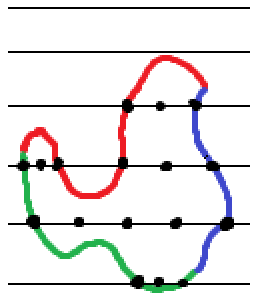
\includegraphics[width=\linewidth]{figures/raycasting_quadrature}
%  \caption{An example raycasting quadrature on a 2D NURBS curve.}
%  \Description{Shows a 2D NURBs curve with horizontal rays intersecting the curve. }
%\end{figure}